\documentclass[addpoints]{exam}

\usepackage{amsmath}
\usepackage{amssymb}
\usepackage{enumitem}
\usepackage{graphicx}
\usepackage{hyperref}
\usepackage{multicol}
\usepackage{tikz}
\usepackage{titling}
\usepackage{tikz}

% Header and footer.
\pagestyle{headandfoot}
\runningheadrule
\runningfootrule
\runningheader{CS 113 Spring 201}{HW 4: Functions, Induction, Graphs}{\theauthor}
\runningfooter{}{Page \thepage\ of \numpages}{}
\firstpageheader{}{}{}

\boxedpoints
\printanswers

\newcommand\union\cup
\newcommand\interx\cap

\graphicspath{{images/}}

\title{Homework 4: Functions, Induction, Graphs}
\author{connected-argument}  % replace with your team name
\date{CS/MATH 113 Discrete Mathematics\\Habib University, Spring 2022}

\begin{document}
\maketitle

\begin{questions}

  \section*{Functions}
  
\question[5] Consider these functions from the set of students in a discrete mathematics class. Under what conditions is the
  function one-to-one if it assigns to every student,
  
  \begin{enumerate}[label=\alph*)]
  \item their mobile phone number.
    \begin{solution}
      This function will normally be one to one as each student will have a different unique mobile phone number, unless 
      two students use or have the same phone number for some reason.
    \end{solution}
  \item their student identification number.
    \begin{solution}
      This will be a one to one function as each student will have had been assigned a unique identification number by the institute.
    \end{solution}
  \item their final grade in the class.
    \begin{solution}
      This will not be one to one function as two or more students can have the same grade. So unless the number of students is less 
      than or equal to the total possible grades, this will not be one to one.
    \end{solution}
  \item their home town.
    \begin{solution}
      This function will usually not be one to one as it is very likely that two or more students in the same class will be from 
      the same hometown. So unless each student is from a different hometown, this will not be one to one.
    \end{solution}
  \item their Ehsas hour appointment.
    \begin{solution}
      This function will be one to one function as each student will be given a different time for appointment, unless group 
      appointments are allowed in which case it will no longer be one to one.
    \end{solution}
  \end{enumerate}


\question[5] If $f$ and $f \circ g$ are one-to-one, does it follow that $g$ is one-to-one? Justify your answer.
  \begin{solution}\\
    Let $f$ be a function from C to D, and and $f \circ g$ be the composition of functions $f$ and $g$, such that $g$ is a function from A to B, 
    then the range of $f$ is a subset of the domain of $f$. We know that $f$ and $f \circ g$ are one-to-one, which means for all a,b in C, 
    $f(a)=f(b)$ if and only if $a = b$, and for all c,d in A, $f \circ g(c)=f \circ g(d)$ if and only if $c = d$\\
    Proof by contradiction:\\
    Suppose $g$ is not one-to-one, i.e, at least two elements in A map to at least one element in B. This means that at least one element in 
    the domain of $f$ has at least two preimages in the range of $g$. By the definition of composition, for $f \circ g$, the preimage of some element 
    in the range of g is also the preimage of some element in the range of $f \circ g$, 
    now since $g$ is not one-to-one, at least one element in $f \circ g$ must have two preimages in the domain of $g$.
    However, we know that $f \circ g$ is one-to-one. There arises a contradiction and our supposition must be wrong. Hence, $g$ must also be one-to-one.\\
    Direct proof:\\
    $g(a) = g(b) \rightarrow a = b$\\
    Let,    \\
    $g(a) = g(b)$\\
    Applying function $f$\\
            $f(g(a)) = f(g(b))$\\
            $f \circ g (a) = f \circ g (b)$\\
    Since $f \circ g$ is one-to-one,\\
            $a = b$\\
    hence proven.
  \end{solution}

\question[5] Prove that a strictly decreasing function from $\mathbb{R}$ to itself is one-to-one. Give an example of a decreasing function from $\mathbb{R}$ to itself that is not one-to-one.
  \begin{solution}
    For strictly decreasing, $f(x) = f(y)$ if and only if $x = y$. Contrapositively, if $x \neq y$, then $f(x) \neq f(y)$.
    So then either $x < y$ or $x > y$.
    If $x < y$, then $f(x) > f(y)$ by the definition of strictly decreasing function. Similarly if $x > y$, then $f(x) < f(y)$ by
    the definition of strictly decreasing function. Therefore $f(x) \neq f(y)$ when $x \neq y$. So for $f(x) = f(y)$ to be true,
    $x$ must be equal to $y$. Therefore a strictly decreasing function from $\mathbb{R}$ to itself must be one to one. \\
    An example of a decreasing function that is not one to one can be $f(x) = - |x|$ as for $x > y$, $f(x) \le f(y)$.
  \end{solution}
  
  \section*{Graphs}
  
\question To lift the spirits of the students on their return, Habib University has decided to build 4 new courtyards--Nature, Ice, Light, and Darkness. Designs are invited and bids are received for the courtyards from 4 architect firms as follows. Parveen Prime can design Nature, Light, and Darkness; Queen Quratulain can design Ice and Light; Reena Rani can design Light and Darkness; and Super Sonam can design Nature and Ice.
  \begin{parts}
  \part[5] Use a bipartite graph to model the four architects and the courtyards that they can design.
    \begin{solution}
      \usetikzlibrary{positioning,chains,fit,shapes,calc}
      \definecolor{myblue}{RGB}{80,80,160}
      \definecolor{mygreen}{RGB}{80,160,80}
      
      \begin{tikzpicture}[thick,
        fsnode/.style={draw,circle},
        ssnode/.style={draw,circle},
        fsnode/.style={fill=myblue},
        ssnode/.style={fill=mygreen},
        % every fit/.style={ellipse,draw,inner sep=-2pt,text width=5cm},
        % ->,shorten >= 3pt,shorten <= 3pt
]      
      % the vertices of U
      \begin{scope}
        [start chain=going below,node distance=9mm]
        \node[fsnode,on chain] (Parveen Prime) [label=left: Parveen Prime] {};
        \node[fsnode,on chain] (Queen Quratulain) [label=left: Queen Quratulain] {};
        \node[fsnode,on chain] (Reena Rani) [label=left: Reena Rani] {};
        \node[fsnode,on chain] (Super Sonam) [label=left: Super Sonam] {};
      \end{scope}

      % the vertices of V
      \begin{scope}
        [xshift=7cm,start chain=going below,node distance=9mm]
        \node[ssnode,on chain] (Nature) [label=right: Nature] {};
        \node[ssnode,on chain] (Ice) [label=right: Ice] {};
        \node[ssnode,on chain] (Light) [label=right: Light] {};
        \node[ssnode,on chain] (Darkness) [label=right: Darkness] {};
      \end{scope}

      % the set U
      \node [myblue,fit=(Parveen Prime) (Super Sonam),label=above:$architects$] {};
      % the set V
      \node [mygreen,fit=(Nature) (Darkness),label=above:$courtyards$] {};

      % the edges
      \draw (Parveen Prime) -- (Nature);
      \draw (Parveen Prime) -- (Light);
      \draw (Parveen Prime) -- (Darkness);
      \draw (Queen Quratulain) -- (Ice);
      \draw (Queen Quratulain) -- (Light);
      \draw (Reena Rani) -- (Light);
      \draw (Reena Rani) -- (Darkness);
      \draw (Super Sonam) -- (Nature);
      \draw (Super Sonam) -- (Ice);
      \end{tikzpicture}
    \end{solution}
    
  \part[5] Use Hall’s theorem to determine whether there is an assignment of architects to courtyards so that each architect is assigned one courtyard to design.
    \begin{solution}\\
      Hall's marriage theorem states, \\
      The bipartite graph $G=(V,E)$ with bipartition (V1, V2) has a complete matching from V1 to V2 if and only if 
$|N(A)|$ is greater than or equals to |A| for all subsets A of V1.\\
      Here, there will be 16 subsets of V1 (architects). Following are the subsets of architects along woth thier cardinality and the cardinality of their neighborhood:\\
    {Parveen Prime} (1) = 3\\
    {Queen Quratulain} (1) = 2\\
    {Reena Rani} (1) = 2 \\
    {Super Sonam} (1) = 2\\
    {Parveen Prime, Queen Quratulain} (2) = 4\\
    {Parveen Prime, Reena Rani} (2) = 3\\
    {Parveen Prime, Super Sonam} (2) = 4\\
    {Queen Quratulain, Reena Rani} (2) = 3 \\
    {Queen Quratulain, Super Sonam} (2) = 3\\
    {Reena Rani, Super Sonam} (2) = 4\\
    {Parveen Prime, Queen Quratulain, Reena Rani} (3) = 4\\
    {Parveen Prime, Queen Quratulain, Super Sonam} (3) = 4\\
    {Parveen Prime, Reena Rani, Super Sonam} (3) = 4\\
    {Queen Quratulain, Reena Rani, Super Sonam} (3) = 4\\
    {Parveen Prime, Queen Quratulain, Reena Rani, Super Sonam} (4) = 4 \\
    Hence, Hall's marriage theorem is passed and there can be a complete matching from architects to courtyards.\\
    \end{solution}

  \part[5] Provide the assignment, if it exists, of architects to courtyards such that each architect is assigned to a courtyard that she can design.
    \begin{solution}
      Parveen Prime $-->$ Darkness\\
      Queen Quratulain $-->$ Ice\\
      Reena Rani $-->$ Light\\
      Super Sonam $-->$ Nature\\

    \end{solution}
  \end{parts}
  
\question  The simple graphs $G_1 = (V_1,E_1)$ and $G_2 = (V_2,E_2$) are \textit{isomorphic} if there exists a one-to-one and onto function $f$ from $V_1$ to $V_2$ with the property that $a$ and $b$ are adjacent in $G_1$ if and only if $f(a)$ and $f(b)$ are adjacent in $G_2$, for all $a$ and $b$ in $V_1$. Such a function $f$ is called an \textit{isomorphism}. Two simple graphs that are not isomorphic are called \textit{non-isomorphic}.

  In other words, when two simple graphs are isomorphic, there is a one-to-one correspondence between the vertices of the two graphs that preserves the adjacency relationship. Isomorphism of simple graphs is an equivalence relation.

  Determine which of the following pairs of graphs are isomorphic. For each pair of graphs, provide an isomorphism (a bijection between the vertices of the graphs) or a rigorous argument that no such bijection exists.

  \begin{tabular}{cccc}
    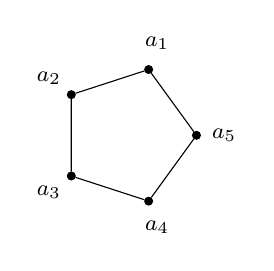
\begin{tikzpicture}
      \tikzstyle{node} = [draw,circle,fill=black,inner sep=1pt]
      \foreach \a in {1,2,...,5}{
        \draw (\a*360/5: 25pt) node(\a)[node]{};
        \draw (\a*360/5: 35pt) node{\footnotesize $a_\a$};
      }
      \path[draw] (1) -- (2) -- (3) -- (4) -- (5) -- (1);
    \end{tikzpicture}
    &
      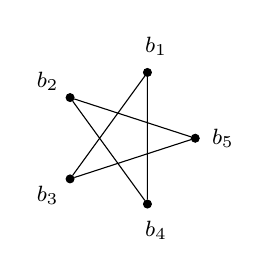
\begin{tikzpicture}
        \tikzstyle{node} = [draw,circle,fill=black,inner sep=1pt]
        \foreach \a in {1,2,...,5}{
          \draw (\a*360/5: 25pt) node(\a)[node]{};
          \draw (\a*360/5: 35pt) node{\footnotesize $b_\a$};
        }
        \path[draw] (2) -- (5) -- (3) -- (1) -- (4) -- (2);
      \end{tikzpicture}
    &
      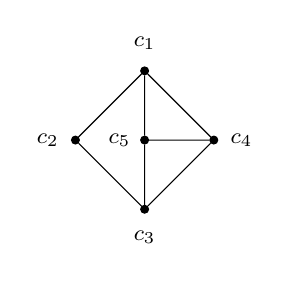
\begin{tikzpicture}
        \tikzstyle{node} = [draw,circle,fill=black,inner sep=1pt]
        \foreach \a in {1,2,...,4}{
          \draw (\a*360/4: 25pt) node(\a)[node]{};
          \draw (\a*360/4: 35pt) node{\footnotesize $c_\a$};
        }
        \node [node, label = left:\footnotesize $c_5$] (5) at (0,0) {};
        \path[draw] (1) -- (2) -- (3) -- (4) -- (1) -- (5) -- (4) -- (3) -- (5);
      \end{tikzpicture}
    &
      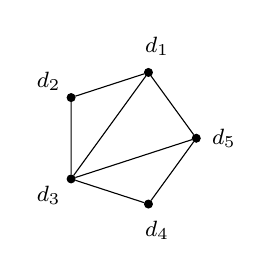
\begin{tikzpicture}
        \tikzstyle{node} = [draw,circle,fill=black,inner sep=1pt]
        \foreach \a in {1,2,...,5}{
          \draw (\a*360/5: 25pt) node(\a)[node]{};
          \draw (\a*360/5: 35pt) node{\footnotesize $d_\a$};
        }
        \path[draw] (1) -- (2) -- (3) -- (4) -- (5) -- (1) -- (3) -- (5);
      \end{tikzpicture}\\
    Graph A & Graph B & Graph C & Graph D    
  \end{tabular}    

  \begin{parts}
  \part[5] Graph A and Graph B
    \begin{solution}
      Yes this pair is isomorphic. A possibility can be $f(a_1) = b_1, \; f(a_2) = b_3, \; f(a_5) = b_4, \; f(a_3) = b_5, \; f(a_4) = b_2$.
    \end{solution}

  \part[5] Graph A and Graph C
    \begin{solution}
      This pair is not isomorphic as in Graph C, the maximum degree is 3 which is not true for Graph A that has degree 2.
    \end{solution}
    
  \part[5] Graph A and Graph D
    \begin{solution}
      This pair is not isomorphic as in Graph D, the maximum degree is 4 which is not true for Graph B that has degree 2.
    \end{solution}
    
  \part[5] Graph B and Graph C
    \begin{solution}
      This pair is not isomorphic as in Graph C, the maximum degree is 3 which is not true for Graph B that has degree 2.
    \end{solution}
    
  \part[5] Graph B and Graph D
    \begin{solution}
      This pair is not isomorphic as in Graph D, the maximum degree is 4 which is not true for Graph B that has degree 2.
    \end{solution}
    
  \part[5] Graph C and Graph D
    \begin{solution}
      This pair is not isomorphic as in Graph D, the maxmium degree is 4 which is not true for Graph C that has degree 3.
    \end{solution}
  \end{parts}

\question[5] Show that in a simple graph with at least two vertices there must be two vertices that have the same degree.
  \begin{solution}\\
    A simple graph is an undirected graph with only one edge between two distinct vertices and has no loops.\\
    Proof by contradiction:\\
    Suppose that in a graph with at least two vertcies, there does not exist any two vertices with the same degree.\\
    Since it is a simple graph, the possible amount of degrees the graph can have is D = $\{0,1,...,n-1\}$. For none of the vertices to 
    have the same degree, every vertex should have a distinct degree from the n possibilities in D. However, if there is a one-to-one correspondence
    between the the set of all vertices V and the possibilities of degrees D, then there arisesa contradiction. If one vertex has a degree of, then another
    vertex cannot have degree of n-1 simultaneously. This means that there cannot exist a one-to-one correspondence, and at least two vertices
    have to have the same degree for it to be a simple graph. 


  \end{solution}
  
\question[5] The \textit{complementary graph} $\overline{G}$ of a simple graph $G$ has the same vertices as  $G$. Two vertices are adjacent in $\overline{G}$ if and only if they are not adjacent in $G$. Given $G$ with $v$ vertices and $e$ edges, how many edges are there in $\overline{G}$? Justify your answer.
  \begin{solution}
    $\overline{G}$ has all vertices in $G$ but all edges that do not exist in $G$. Thus the number of edges in $\overline{G}$ can
    be found by subtracting the number of edges $e$ in $G$ from total possible edges that can be made in the graph $G$. For $v$ 
    vertices in a simple graph $G$, each vertex can have $v-1$ possible edges. So total possible edges for $v$ vertices become $v$ number 
    of edges times total possible edges for each vertex which is $v(v-1)$. However, this means that each edge will have been counted
    twice, thus the total possible edges will be divided by 2 to compensate the doubled counting. Then the total number of possible edges
    become $\dfrac{v(v-1)}{2}$. A simple graph $G$ has $e$ edges and its complement $\overline{G}$ will have those edges that do not 
    exist in $G$. So $\overline{G}$ will have the remaining edges that are $\dfrac{v(v-1)}{2} - e$ number of edges where $v$ 
    is the number of vertices and $e$ is the number of edges in a simple graph $G$. 
  \end{solution}
  
  \section*{Induction}
  
\question Prove the following using induction.
  \begin{parts}
  \part[5] Given a a relation $R$ that is reflexive and transitive, $R^n = R$ for all positive integers $n$.
    \begin{solution}
      (Proof by mathematical induction) \\
      \textbf{Base Case: } For $n = 1$, $R^1 = R$ which is trivially true. \\
      \textbf{Inductive Hypothesis: } Suppose that $R^n = R$ is true. (This is the inductive hypothesis) \\
      \textbf{Inductive Step: } $R^{n+1} = R$. By definition of composite relations, $R^{n+1} = R^n \circ R$. Then, $R^n \circ R \subseteq R$ and $R \subseteq R^n \circ R$. \\
      \underline{Transitive: } For $(a, c) \in R^n \circ R$, there must be an element $b$ such that $(a, b) \in R$ and $(b, c) \in R^n$. Then by the inductive hypothesis, 
      $(b, c) \in R$ and $(a, b) \in R^n$. Since R is transitive, $(a, c) \in R$. Since $(a, c) \in R^n \circ R$, therefore proved that $R \subseteq R^n \circ  R$ and $R^n \circ R \subseteq R$. Hence $R^n = R$. \\
      
      \underline{Reflexive: } $\forall a \in A$, $(a, a) \in R$ and $(a, a) \in R^n$ by the inductive hypothesis. Then by definition of composite relations, 
      $(a, a) \in R^n \circ R$. Therefore, $R^n \circ R \subseteq R$ and $R \subseteq R^n \circ R$. Thus proved that $R^n = R$.
    \end{solution}

  \part[5] A relation $R$ on a set $A$ is transitive if and only if $R^n \subseteq R$ for all positive integers $n$.
    \begin{solution}
      \textbf{\underline{IF:}} Suppose that $R^n \subseteq R$ for all positive integers $n$. Then for the base case, $R^2 \subseteq R$.
      If $(a, b) \in R$ and $(b, c) \in R$, then by definition of composition, $(a, c) \in R^2$. Since $R^2 \subseteq R$, then 
      $(a, c) \in R$. Therefore, $R$ is transitive. \\
      \textbf{\underline{Only IF:}} \\
      (Proof by mathematical induction)\\
      \textbf{Base case: } For $n = 1$, $R^1 \subseteq R$, which is trivially true. \\
      \textbf{Inductive Hypothesis: } Suppose $R^n \subseteq R$ is true. (This is the inductive hypothesis) \\
      \textbf{Inductive Step: } For $n + 1$, $R^{n+1} \subseteq R$. By definition of composition, $R^{n+1} = R^n \circ R$. Assume 
      that $(a, c) \in R^{n+1}$. Then because $R^{n+1} = R^n \circ R$, there exists an element $b$ such that $(a, b) \in R$ and $(b, c) \in R^n$. 
      Then the inductive hypothesis implies that $(b, c) \in R$. Moreover, since $R$ is transitive, and $(a, b) \in R$, and $(b, c) \in R$, then 
      $(a, c) \in R$ as well. Since $(a, c) \in R$ and $(a, c) \in R^{n+1}$, this shows that $R^{n+1} \subseteq R$. \\
      Hence proved.
    \end{solution}
  \end{parts}


\question[5] Prove via induction that a complete graph with $n$ vertices contains $\dfrac{n(n-1)}{2}$ edges.
  \begin{solution}
    Let $S(n) = \dfrac{n(n-1)}{2}$ \\
    \textbf{Base Case (n = 1):} $S(1) = \dfrac{1(1-1)}{2} = 0$. This is true as a complete graph with 1 vertex will have 0 edges. \\
    \textbf{Inductive Hypothesis (n = k):} Suppose that our statement is true for $n = k$. Then $S(k) = \dfrac{k(k-1)}{2}$ edges. \\
    \textbf{Inductive Step (n = k + 1):} Then for $n = k + 1$, there should be $S(k + 1) = \dfrac{(k+1)(k+1-1)}{2} = \dfrac{k(k+1)}{2}$ edges. \\
    $S(k+1)$ has $S(k)$ edges + total edges by adding one more vertex. In a complete graph, each vertex is connected to all other vertices,
    therefore adding 1 vertex introduces $k$ edges where $k$ is the number of existing nodes in the graph. $k$ edges are added on adding one node as 
    that node is then connected to $k$ other nodes, thus $k$ edges are added.
    Then $S(k+1) = S(k) + k$. \\
    $\implies S(k + 1) = \dfrac{k(k-1)}{2} + k$ \\
    $\implies S(k + 1) = \dfrac{k^2 - k + 2k}{2}$ \\
    $\implies S(k + 1) = \dfrac{k^2 + k}{2}$ \\
    $\implies S(k + 1) = \dfrac{k(k + 1)}{2}$. \\
    Therefore we arrive at the same conclusion that was needed, and thus the statement has been proved by induction.
  \end{solution}
  
\end{questions}
\end{document}


%%% Local Variables:
%%% mode: latex
%%% TeX-master: t
%%% End:
